\begin{figure*}[h]
\centering
%\subfigure[]
%{
%	\label{fig:multi_berkeley_random_hum}
%	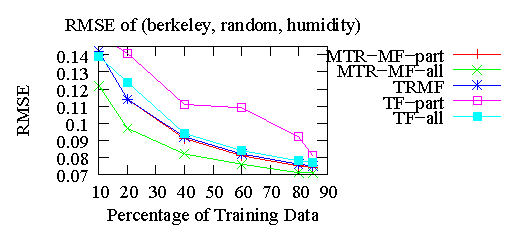
\includegraphics[scale=1]{berkeley_random_humidity_pspdftex.eps}
%}
%\hspace{0in}
%\subfigure[]
%{
%	\label{fig:multi_berkeley_random_tem}
%	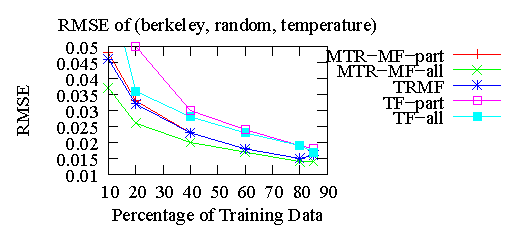
\includegraphics[scale=1]{berkeley_random_temperature_pspdftex.eps}
%}
%\hspace{0in}
%\subfigure[]
%{
%	\label{fig:multi_berkeley_temporal_hum}
%	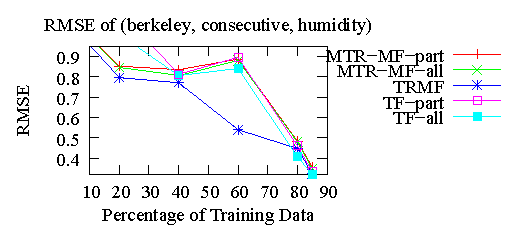
\includegraphics[scale=1]{berkeley_temporal_humidity_pspdftex.eps}
%}
%\hspace{0in}
%\subfigure[]
%{
%	\label{fig:multi_berkeley_temporal_tem}
%	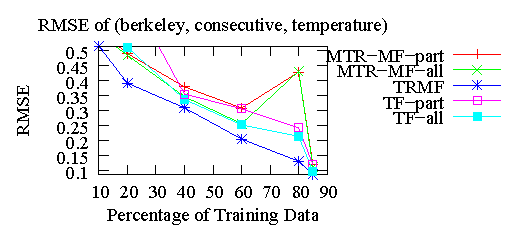
\includegraphics[scale=1]{berkeley_temporal_temperature_pspdftex.eps}
%}
\hspace{0in}
\subfigure%[]
{
	\label{fig:multi_traffic_random_hum}
	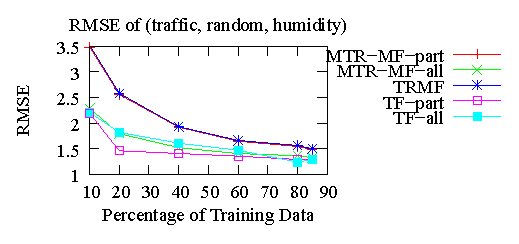
\includegraphics[height=2.6cm, trim=15 0 0 0, clip]{traffic_random_humidity_pspdftex.eps}
}
\hspace{0in}
\subfigure%[]
{
	\label{fig:multi_traffic_random_tem}
	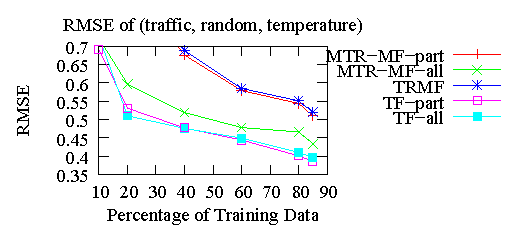
\includegraphics[height=2.6cm, trim=15 0 0 0, clip]{traffic_random_temperature_pspdftex.eps}
}
\hspace{0in}
\subfigure%[]
{
	\label{fig:multi_traffic_temporal_hum}
	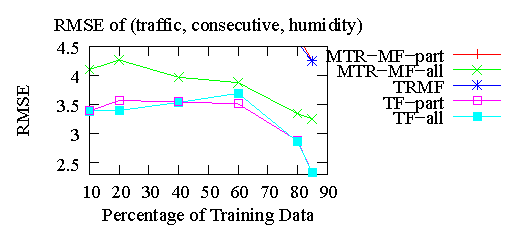
\includegraphics[height=2.6cm, trim=15 0 0 0, clip]{traffic_temporal_humidity_pspdftex.eps}
}
\hspace{0in}
\subfigure%[]
{
	\label{fig:multi_traffic_temporal_tem}
	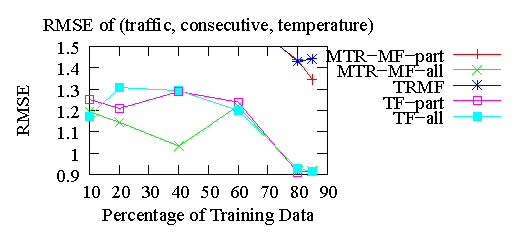
\includegraphics[height=2.6cm, trim=15 0 0 0, clip]{traffic_temporal_temperature_pspdftex.eps}
}
\vspace{-0.1in}

\caption{\label{fig:multi}
Accuracy of Multivariate models, varying the percentage of training data}
\vspace{-0.05in}
%\hspace{0in}






%\caption{}
\end{figure*}
















%\begin{table*}
%%
%\begin{tabular}{cc}
%\subfigure[A]{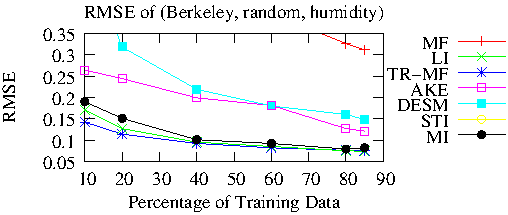
\includegraphics[scale=1]{table2_BRH}} 
%   & \subfigure[B]{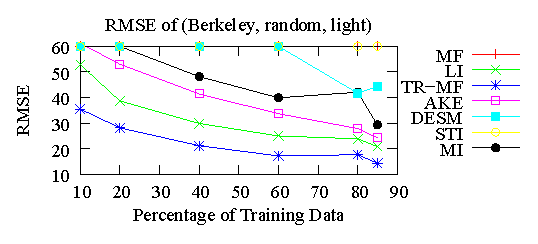
\includegraphics[scale=1]{table3_BRL}}\\
%\end{tabularx}
%\end{table*}
%\end{figure}
%\begin{figure}[H]
%\centering
%\mbox{
%\input{table11.pspdftex}}
%\caption{RMSE of (traffic, temporal, temperature}
%\end{figure}
